We have seen in Section~\ref{sec:coordination:bp} that the Loopy Belief
Propagation program can obtain significant benefits from using different
evaluation strategies due to the inherient non-determinism of LBP.  The proposed
asynchronous approach has shown to be an improvement over the synchronous
version because it leads to faster convergence time. An improved evaluation
strategy is the Splash Belief
Propagation~(SBP)~\cite{Gonzalez+al:aistats09paraml}, where belief values are
computed by first building a tree and then updating the beliefs of each node
twice, first from the leaves to the root and then from the root to the leaves
These \emph{splash trees} are built by starting at a node whose belief changed
the most in the last update. The trees must be built iteratively until
convergence is achieved.

In an environment with $T$ threads, it is then possible to build $T$ splash
trees concurrently. First, we partition the nodes into $T$ regions and then
assign each region to a thread. A thread is then responsible for iteratively
building splash trees on that region until convergence is reached.
Fig.~\ref{fig:threads:splash_bp} shows a grid of nodes that has been partitioned
in two regions where splash trees will be built. To build a splash tree, a
thread starts from the highest priority node (the tree's root) from its region
and then performs a breadth-first search from that node to construct the rest of
the tree. The belief values are then computed in order.

\begin{figure}[ht]
   \begin{center}
      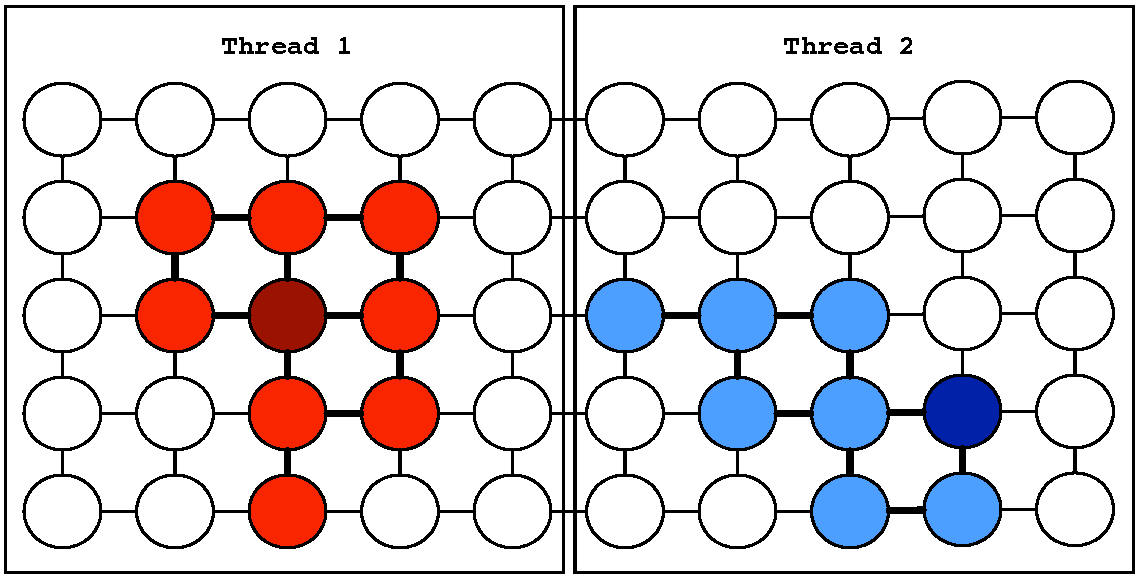
\includegraphics[width=0.7\linewidth]{figures/threads/splash_bp}
   \end{center}
   \caption{Creating splash trees using multiple threads. The graph is
      partitioned into two regions and each thread is able to build separate
   splash trees starting from the highest priority node.}
   \label{fig:threads:splash_bp}
\end{figure}

The LM implementation for SBP is shown in Fig.~\ref{code:threads:sbp} shows the
LM implementation. First, in lines
\ref{line:threads:splash_part1}-\ref{line:threads:splash_part2}, we partition
the nodes into regions using \code{set-thread} and then we start the creation of
the first splash tree (line~\ref{line:threads:splash_first}) by deriving
\code{start-tree(T)}.  The remaining phases of the algorithm are explained as
follows:

\begin{figure}[!htb]
\begin{Verbatim}[numbers=left,commandchars=*\{\},fontsize=\codesize]
type list node tree.

type linear partitioning(thread, int). // Number of nodes to receive.
type linear start-tree(thread).
type linear new-tree(thread, tree, tree).
type linear expand-tree(thread, tree).
type linear first-phase(thread, tree, tree).
type linear second-phase(thread, tree).
type linear start(node).

start(A).
partitioning(T, @world / @threads). // Move @world/@threads nodes.

!coord(A, X, Y), start(A) // Moving this node.*label{line:threads:splash_part1}
   -o set-static(A), set-thread(A, grid(X, Y)).
just-moved(A), partitioning(T, Left) // Thread received another node.
   -o partitioning(T, Left - 1).
partitioning(T, 0) -o start-tree(T).*label{line:threads:splash_part2}*label{line:threads:splash_first}

start-tree(T),*label{line:threads:splash_building1} priority(A, P), P > 0.0 *hfill{} // Tree building
   -o priority(A, P), expand-tree(T, [A], []).*label{line:threads:splash_building2}
expand-tree(T, [A | All], Next)
   -o thread-id(A, Id),
      [collect => L | !edge(A, L), ~ L in All, ~ L in Next,*label{line:threads:splash_agg1} priority(L, P), P > 0.0,
         thread-id(L, Id2), Id1 = Id2 | priority(L, P), thread-id(L, Id2) |
         new-tree(T, [A | All],
            if len(All) + 1 >= maxnodes then [] else Next ++ L end)].*label{line:threads:splash_agg2}*label{line:threads:splash_next}

new-tree(T, [A | All], [])
   -o schedule-next(A), first-phase(T, reverse([A | All]), [A | All]).*label{line:threads:splash_first_phase}
new-tree(T, All, [B | Next])
   -o schedule-next(B), expand-tree(T, [B | All], Next).

first-phase(T, [A], [A]), running(T, A) *hfill{} // First phase
   -o running(T, A), update(A), remove-priority(A), start-tree(T).
first-phase(T, [A, B | Next], [A]), running(T, A)
   -o running(T, A), update(A), schedule-next(B), second-phase(T, [B | Next]).*label{line:threads:splash_first_update1}
first-phase(T, All, [A, B | Next]), running(T, A)
   -o running(T, A), update(A), schedule-next(B), first-phase(T, All, [B | Next]).*label{line:threads:splash_first_update2}

second-phase(T, [A]), running(T, A) *hfill{} // Second phase
   -o running(T, A), update(A), remove-priority(A), start-tree(T).*label{line:threads:splash_second_update1}
second-phase(T, [A, B | Next]), running(T, A)
   -o running(T, A), update(A), schedule-next(B), second-phase(T, [B | Next]).*label{line:threads:splash_second_update2}
\end{Verbatim}

   \caption{LM code for the Splash Belief Propagation program.}
  \label{code:threads:sbp}
\end{figure}

\begin{description}

   \item[Tree building]: Tree building starts after the rule in lines
      \ref{line:threads:splash_building1}-\ref{line:threads:splash_building2} is
      derived. Since the thread always picks the higher priority node, we start
      by adding that node to the list that represents the tree. In lines
      \ref{line:threads:splash_agg1}-\ref{line:threads:splash_agg2}, we use an
      aggregate to gather all the neighbor nodes that have a positive priority
      (due to a new belief update) and are in the same thread. Nodes are
      collected into list \code{L} and appended to list \code{Next}
      (line~\ref{line:threads:splash_next}).

   \item[First phase]: When the number of nodes in the tree reaches a certain
      limit, a \code{first-phase} is generated to update the beliefs of all
      nodes in the tree (line~\ref{line:threads:splash_first_phase}). As the
      nodes are updated, starting from the leaves and ending at the root, an
      \code{update} fact is derived to update the belief values
      (lines~\ref{line:threads:splash_first_update1}
      and~\ref{line:threads:splash_first_update2}).

   \item[Second phase]: The computation of beliefs is performed from the root to
      the leaves and the belief values are updated a second time
      (lines~\ref{line:threads:splash_second_update1}
      and~\ref{line:threads:splash_second_update2}).

\end{description}

SBP is also implemented in GraphLab~\cite{GraphLab2010}, a C++ framework for
writing machine learning algorithms. GraphLab provides the splash scheduler as
part of its framework. We measured the behavior of LBP and SBP for both LM and
GraphLab. Fig.~\ref{results:splash_bp} shows that both systems have very similar
behavior when using a variable number of threads, but for higher number of
threads and, in particular, for more than 15 threads, LM shows better speedups
than GraphLab. In terms of running times, LM is, on average, 1.4 times slower
than GraphLab, although LM program code is more concise.
